\documentclass{../ucll-slides}
\usepackage{../pvm}
\usepackage{siunitx}
\usepackage{ifthen}

\usetikzlibrary{decorations.pathmorphing}

\pgfdeclaredecoration{penciline}{initial}{
  \state{initial}[width=+\pgfdecoratedinputsegmentremainingdistance,
    auto corner on length=1pt,
  ]{
    \ifthenelse
        {\pgfkeysvalueof{/tikz/penciline/jag ratio}=0} {
          \pgfpathcurveto%
              {% 1st control point
                \pgfpoint
                    {\pgfdecoratedinputsegmentremainingdistance/2}
                    {2*rnd*\pgfdecorationsegmentamplitude}
              }
              {%% 2nd control point
                \pgfpoint
                %% Make sure random number is always between origin and target points
                    {\pgfdecoratedinputsegmentremainingdistance/2}
                    {2*rnd*\pgfdecorationsegmentamplitude}
              }
              {% 2nd point (1st one is implicit)
                \pgfpointadd
                    {\pgfpointdecoratedinputsegmentlast}
                    {\pgfpoint{0*rand*1pt}{0*rand*1pt}}
              }          
        } {
          \pgfpathcurveto%
              {% 1st control point
                \pgfpoint
                    {\pgfdecoratedinputsegmentremainingdistance*rnd*1pt}
                    {\pgfkeysvalueof{/tikz/penciline/jag ratio}*
                      rand*\pgfdecorationsegmentamplitude}
              }
              {%% 2nd control point
                \pgfpoint
                %% Make sure random number is always between origin and target points
                    {(.5+0.25*rand)*\pgfdecoratedinputsegmentremainingdistance}
                    {\pgfkeysvalueof{/tikz/penciline/jag ratio}*
                      rand*\pgfdecorationsegmentamplitude}
              }
              {% 2nd point (1st one is implicit)
                \pgfpointadd
                    {\pgfpointdecoratedinputsegmentlast}
                    {\pgfpoint{rand*1pt}{rand*1pt}}
              }
        }
  }
  \state{final}{}
}




\tikzset{
  penciline/.code={\pgfqkeys{/tikz/penciline}{#1}},
  penciline={
    jag ratio/.initial=5,
    decoration/.initial = penciline,
  },
  penciline/.style = {
    decorate,
    penciline/.cd,
    #1,
    /tikz/.cd,
  },
  decorate,
  decoration={\pgfkeysvalueof{/tikz/penciline/decoration}},
}

\title{Data Compression}
\author{Fr\'ed\'eric Vogels}


\begin{document}

\begin{frame}
  \titlepage
\end{frame}

\begin{frame}
  \frametitle{Data Compression}
  \begin{center}
    Encoding same information using less space
  \end{center}

  \begin{center}
    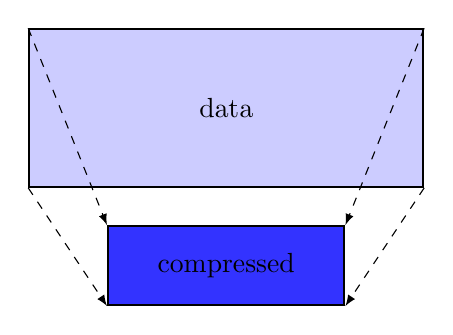
\begin{tikzpicture}[data/.style={draw,thick}]
      \node[data,minimum width=5cm,minimum height=2cm,fill=blue!20] (uncompressed) at (0,0) {data};
      \node[data,minimum width=3cm,minimum height=1cm,fill=blue!80] (compressed) at (0,-2) {compressed};

      \foreach \pos in {north west,north east,south west,south east} {
        \draw[-latex,dashed] (uncompressed.\pos) -- (compressed.\pos);
      }
    \end{tikzpicture}
  \end{center}
\end{frame}

\begin{frame}
  \frametitle{Example: Movie Compression}
  \structure{Audio}
  \begin{itemize}
    \item \link{https://en.wikipedia.org/wiki/Blu-ray}{Dolby TrueHD}
    \item 6 channels, 192kHz, 24 bit
    \item Bitrate: $6 \times \SI{192000}{} \times 24 = \SI{27648000}{bps}$
  \end{itemize}
  \vskip5mm
  \structure{Video}
  \begin{itemize}
    \item \link{https://en.wikipedia.org/wiki/Blu-ray}{Blu-Ray HD video format}
    \item Resolution $1920 \times 1080$, 24fps, 24 bit colours
    \item Bitrate: $1920 \times 1080 \times 24 \times 24 = \SI{1194393600}{bps}$
  \end{itemize}
  \vskip5mm
  \structure{Total}
  \[
    \SI{1222041600}{bps} \approx \SI{146}{MiB/s}
  \]
\end{frame}

\begin{frame}
  \frametitle{Example: Movie Compression}
  \[
    \SI{1222041600}{bps} \approx \SI{146}{MiB/s}
  \]
  \vskip5mm
  \structure{Streaming}
  \begin{itemize}
  \item Streaming uncompressed requires $\SI{1222}{Mbps}$ connection
    \item \link{https://en.wikipedia.org/wiki/List_of_countries_by_Internet_connection_speeds}{Best avg connection speed}: South Korea with $\SI{20.5}{Mbps}$
  \end{itemize}
  \vskip5mm
  \structure{Optical Disc}
  \begin{itemize}
    \item \link{https://en.wikipedia.org/wiki/PlayStation_4_technical_specifications}{PS4} reads discs at \SI{27}{MiB/s}
    \item Size of 120' movie: \SI{8194}{GiB}
    \item \link{https://en.wikipedia.org/wiki/Blu-ray}{Industry Standard}: \SI{50}{Gib} for dual layer disc
  \end{itemize}
\end{frame}

\begin{frame}
  \frametitle{Where is Compression Used?}
  \begin{itemize}
    \item Images: JPEG, PNG, \dots
    \item DVD/BluRay
    \item Music/video streaming
    \item Audio formats MP3, WMA, MA4
    \item Zip, 7z, rar, /\dots
    \item HTTP compression
  \end{itemize}
\end{frame}

\section{Types of Compression}

\frame{\tableofcontents[currentsection]}

\begin{frame}
  \frametitle{Lossless}
  \begin{center}
    \begin{tikzpicture}
      \node[minimum width=3cm,minimum height=2cm,fill=red!25,draw] (uncompressed) at (0,0) {};
      \node[minimum width=2cm,minimum height=1cm,fill=red!75,draw] (compressed) at (5,0) {};

      \coordinate (uc1) at ($ (compressed.west) ! 0.5 ! (compressed.north west) $);
      \coordinate (uc2) at ($ (compressed.west) ! 0.5 ! (compressed.south west) $);
      
      \draw let \p1=(uncompressed.east),
                \p2=(uc1) in
            [-latex] (\x1,\y2) -- (uc1) node[font=\tiny,above,midway] {compress};
      \draw let \p1=(uncompressed.east),
                \p2=(uc2) in
            [-latex] (uc2) -- (\x1,\y2) node[font=\tiny,below,midway] {decompress};
    \end{tikzpicture}
  \end{center}
  \begin{itemize}
    \item Compressing then decompressing yields the original data
    \item No information is lost
    \item Examples: zip, 7z, rar, png
  \end{itemize}
\end{frame}

\begin{frame}
  \frametitle{Lossy}
  \begin{center}
    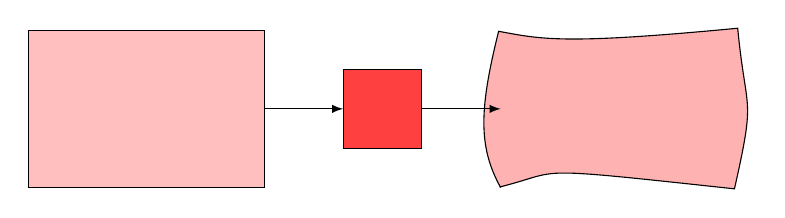
\begin{tikzpicture}
      \draw[fill=red!25] (-4.5,-1) rectangle ++(3,2);
      \draw[fill=red!75] (-.5,-.5) rectangle ++(1,1);
      \draw[fill=red!30,penciline={jag ratio=4}] (1.5,-1) rectangle ++(3,2);

      \draw[-latex] (-1.5,0) -- (-.5,0);
      \draw[-latex] (.5,0) -- (1.5,0);
    \end{tikzpicture}
  \end{center}
  \begin{itemize}
    \item Part of the information is lost
    \item Generally used with sound and images
    \item Examples: jpeg, mp3, DivX, \dots
  \end{itemize}
\end{frame}

\begin{frame}
  \frametitle{Lossy Compression: Images}
  \begin{center}
    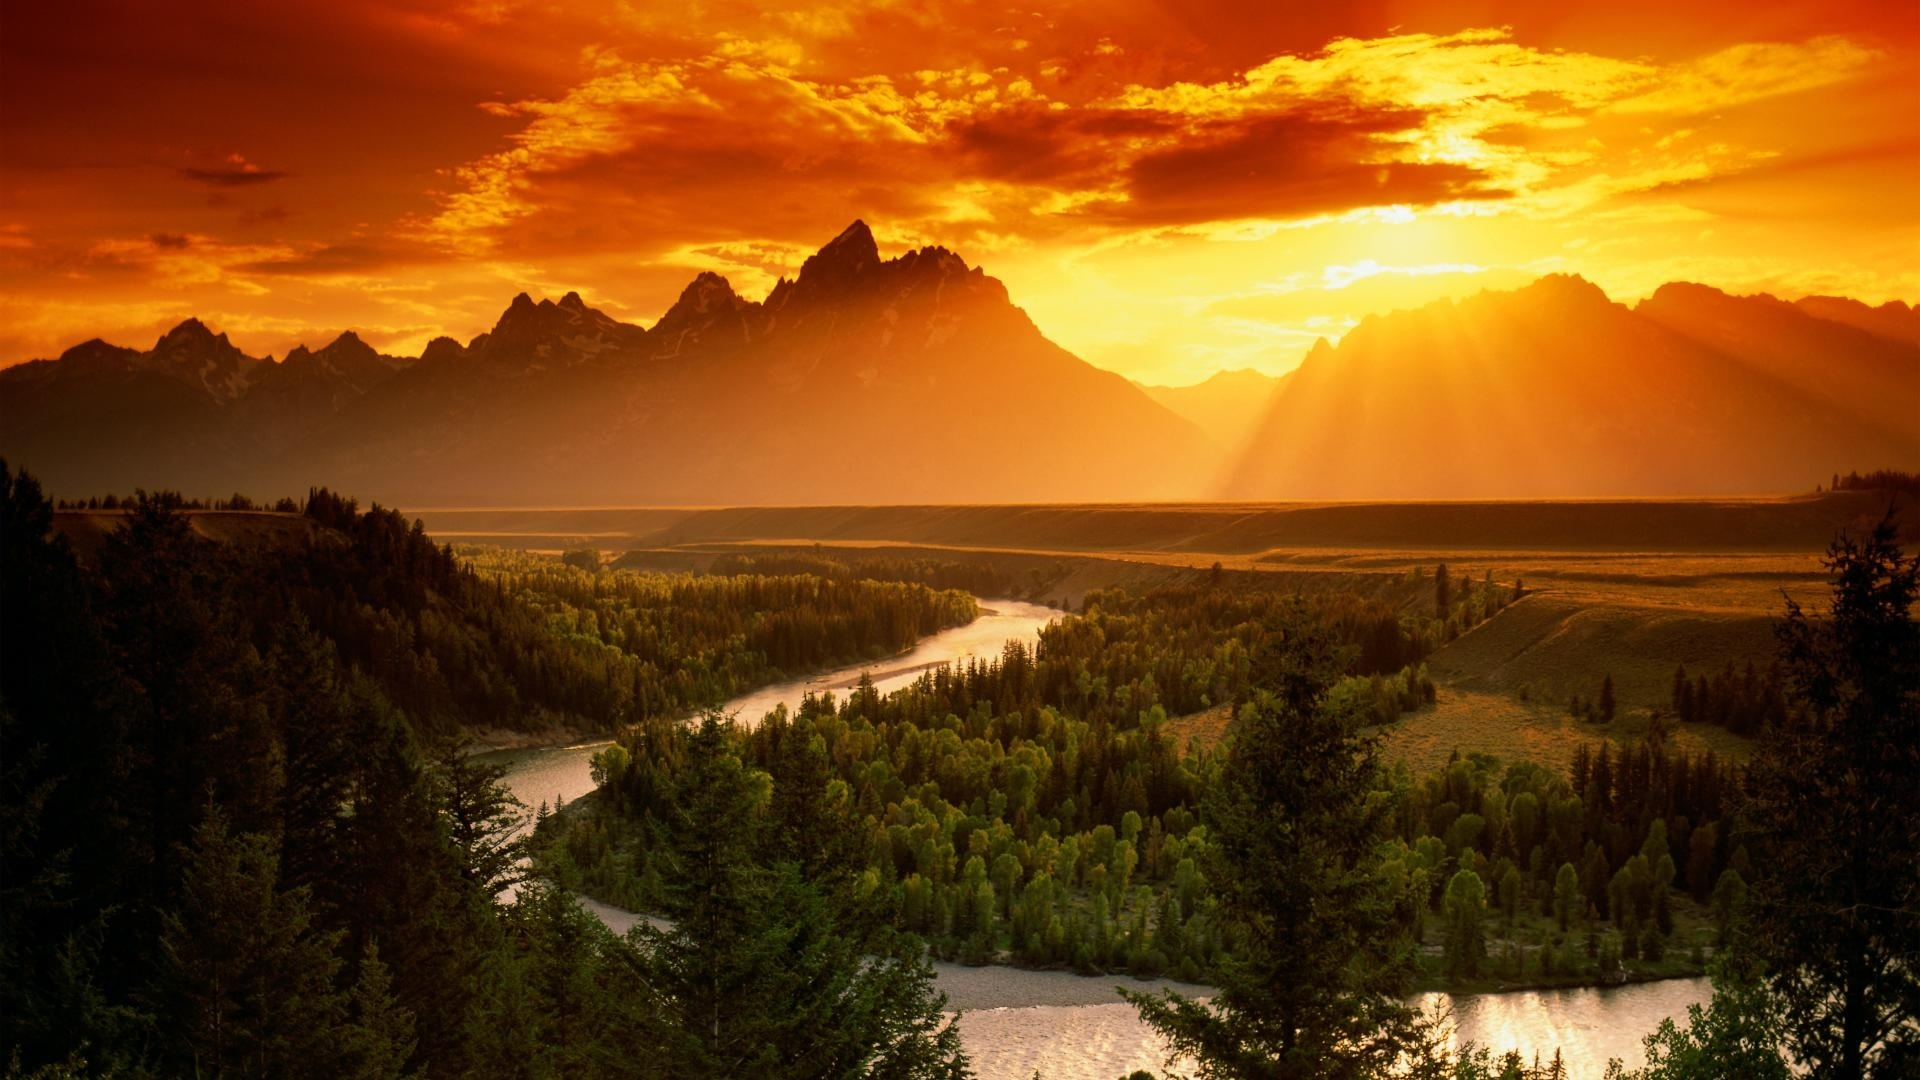
\includegraphics[height=6cm]{lossless.jpg}
  \end{center}
\end{frame}

\begin{frame}
  \frametitle{Lossy Compression: Images}
  \begin{center}
    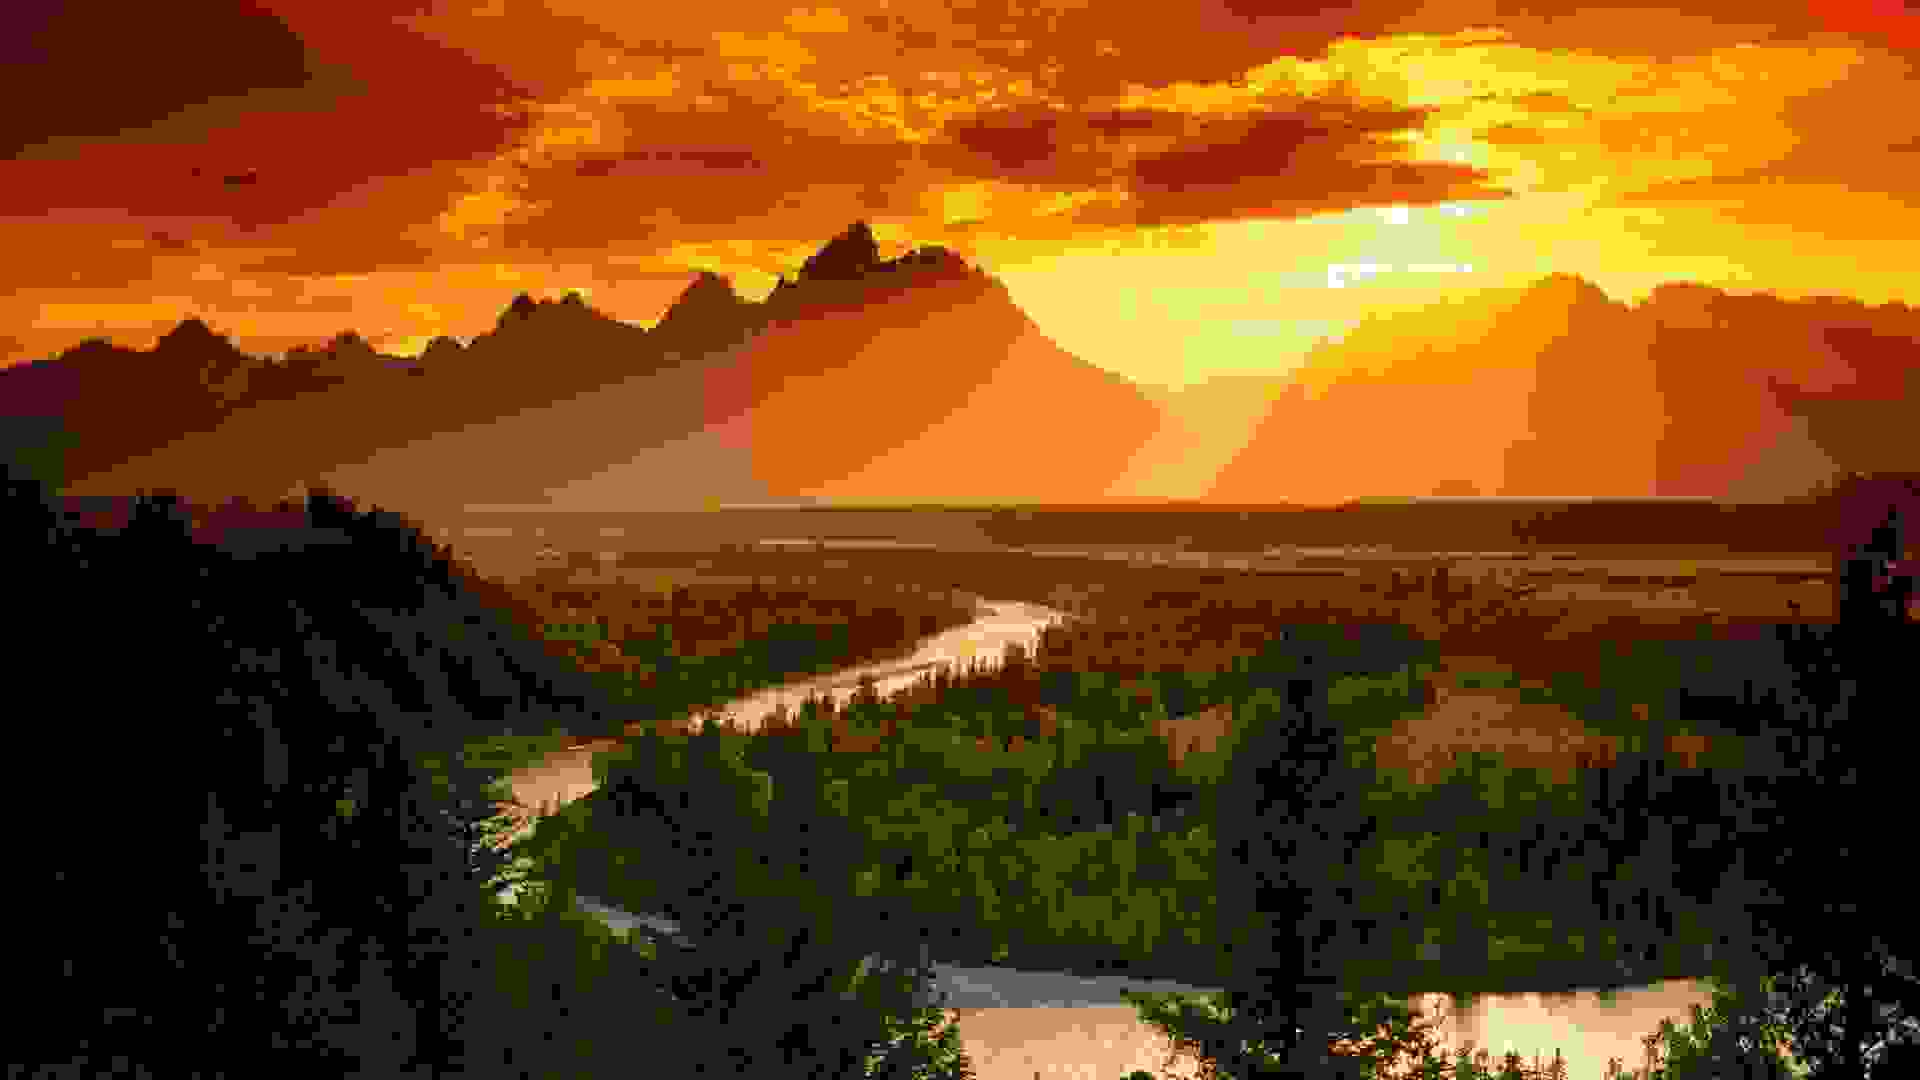
\includegraphics[height=6cm]{lossy.jpg}
  \end{center}
\end{frame}

\begin{frame}
  \frametitle{Lossy Compression: MP3}  
  \begin{itemize}
    \item MP3 takes into account the human ear (\link{https://en.wikipedia.org/wiki/Psychoacoustics}{psychoacoustics})
    \item Uses \link{http://www.mp3-tech.org/tech.html}{several techniques}
          \begin{itemize}
            \item Minimal audition threshold
            \item Masking effect
            \item Joint Stereo coding
            \item Bytes reservoir
            \item Huffman coding
          \end{itemize}
  \end{itemize}
\end{frame}

\begin{frame}
  \frametitle{MP3}
  \begin{center}
    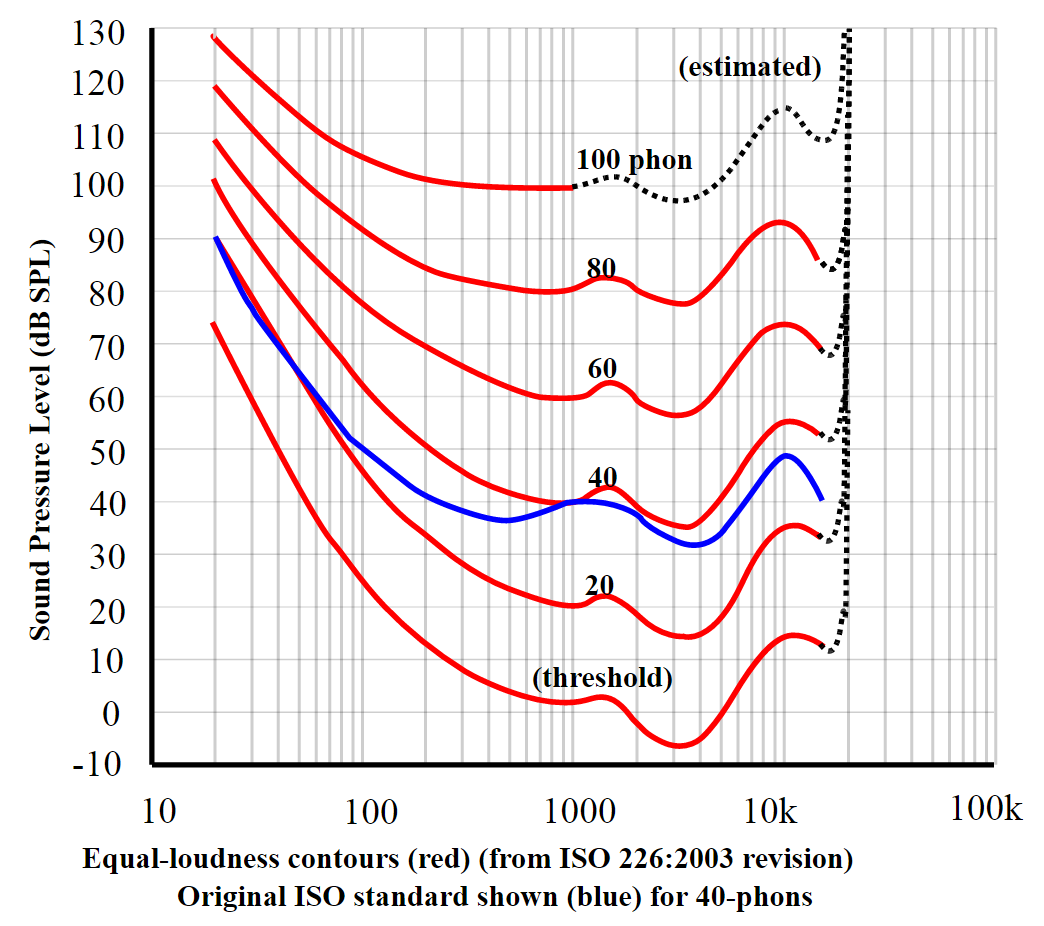
\includegraphics[height=5.5cm]{isophones.png}
  \end{center}
  \begin{itemize}
    \item Our \link{https://en.wikipedia.org/wiki/Equal-loudness_contour}{perception} of loudness depends on the pitch
    \item Lower sounds need more energy to appear loud
    \item MP3 removes sounds that are below a certain loudness
  \end{itemize}
\end{frame}

\begin{frame}
  \frametitle{MP3: Masking Effect}
  \begin{itemize}
    \item Loud noise mask soft noises
    \item Soft noises can be removed
    \item Forward masking: sounds can mask future sounds
    \item \link{https://en.wikipedia.org/wiki/Backward_masking}{Backwards masking}: later sounds can make earlier sounds inaudible
    \item Sounds in the same \link{https://en.wikipedia.org/wiki/Auditory_masking}{critical bandwidth} are merged into a single sound
  \end{itemize}
\end{frame}

\begin{frame}
  \frametitle{MP3: Joint Stereo Encoding}
  \structure{Locating Sounds}
  \begin{itemize}
    \item Humans have two ears: left and right
    \item Brain uses differences in L/R to locate sounds
    \item Human ear fails to locate very low and very high sounds
    \item These sounds can be stored in mono
  \end{itemize}
  \vskip5mm
  \structure{Similarities Between Channels}
  \begin{itemize}
    \item Left and right channels are often similar
    \item Mid/Side instead of Left/Right
    \item Mid contains sounds common to L and R
    \item Side contains differences between L and R
  \end{itemize}
\end{frame}

\begin{frame}
  \frametitle{MP3}
  \structure{Bytes Reservoir}
  \begin{itemize}
    \item Some parts are easy to encode (e.g.\ silent parts)
    \item Some parts require more detail (e.g.\ many instruments)
    \item Spend more bits on detailed parts
  \end{itemize}
  \vskip5mm
  \structure{Final Encoding To Bits}
  \begin{itemize}
    \item Huffman encoding
    \item Will be discussed in detail later
  \end{itemize}
\end{frame}

\end{document}